\section{Numerical Examples}
\subsection{Validation}
As an improved reformulation, in this section, we mainly demonstrate the fact that the proposed formulation is able to produce a desired hardening response.
The cantilever beam has a unit length $L=1$, and all rigidities and yield forces are set to unity, that is, $EA=1$, $EI_z=1$, $P^y=1$ and $M^y_z=1$.
Units are dropped for brevity.
\subsubsection{Isotropic Hardening}
The interaction surface is defined as
\begin{gather}
\Phi=\left(\dfrac{\overline{P}-\overline{\beta}_P}{1+0.1\overline{\alpha}}\right)^2+2\left(\dfrac{\overline{M}_z-\overline{\beta}_{M_z}}{1+0.1\overline{\alpha}}\right)^2-1,
\end{gather}
implying $H=0.1$.
The theoretical hardening ratio can be computed according to \eqsref{eq:nm_eqv_iso_hardening}.
\figref{fig:iso_hardening_a}, \figref{fig:iso_hardening_b} and \figref{fig:iso_hardening_c} present uniaxial cyclic isotropic hardening response under axial force, shear force, and end moment, respectively.
\begin{figure}[htb]
\centering\footnotesize
\includegraphics[page=5]{PICCOLLECTION}
\caption{Isotropic hardening validation for axial force.}\label{fig:iso_hardening_a}
\end{figure}
\begin{figure}[htb]
\centering\footnotesize
\includegraphics[page=6]{PICCOLLECTION}
\caption{Isotropic hardening validation for transverse force.}\label{fig:iso_hardening_b}
\end{figure}
\begin{figure}[htb]
\centering\footnotesize
\includegraphics[page=7]{PICCOLLECTION}
\caption{Isotropic hardening validation for moment.}\label{fig:iso_hardening_c}
\end{figure}
Due to numerical discretisation, some points fall in the transition region(s) and lead to intermediate stiffness values.
They can be ignored.
The desired linear isotropic hardening ratio is properly generated no matter which end yields.
As aforementioned, it is possible to define different hardening functions $h\left(\overline{\alpha}\right)$ for different components to achieve an identical hardening ratio for single DoF loading cases.
However, a unified hardening function ensures the interaction surface grows in size uniformly (isotropic scaling).
\subsubsection{Kinematic Hardening}
The adopted linear kinematic hardening rule is defined as
\begin{gather}
\dot{\overline{\bbeta}}=K\dot{\overline{\be}^p}=0.1\dot{\overline{\be}^p}.
\end{gather}
The theoretical hardening ratio can be computed according to \eqsref{eq:nm_eqv_kin_hardening}.
\figref{fig:kin_hardening_a}, \figref{fig:kin_hardening_b} and \figref{fig:kin_hardening_c} present uniaxial cyclic kinematic hardening response under axial force, shear force, and end moment, respectively.
\begin{figure}[htb]
\centering\footnotesize
\includegraphics[page=8]{PICCOLLECTION}
\caption{Kinematic hardening validation for axial force.}\label{fig:kin_hardening_a}
\end{figure}
\begin{figure}[htb]
\centering\footnotesize
\includegraphics[page=9]{PICCOLLECTION}
\caption{Kinematic hardening validation for transverse force.}\label{fig:kin_hardening_b}
\end{figure}
\begin{figure}[htb]
\centering\footnotesize
\includegraphics[page=10]{PICCOLLECTION}
\caption{Kinematic hardening validation for moment.}\label{fig:kin_hardening_c}
\end{figure}
The target linear kinematic hardening behaviour is also properly generated.
The hardening ratio stays constant (as assigned) for all DoFs, no matter whether one end yields or both ends yield.
\subsection{Calibration}
As mentioned before, in \eqsref{nm:kinematics}, the elemental deformation essentially consists of end-section curvatures and axial strain. It is possible to calibrate the hardening behaviour according to section analysis results in absence of the corresponding experimental data.

An example is presented to show the process by applying moment to a rectangular section.
The section has a geometry of $w\times{}b=12\times1$, the theoretical shape factor of which is \num{1.5}.
This leads to the ultimate moment $M^{ult}=1.5M^y$ assuming material response is purely elastic and perfectly plastic.
By choosing material yield stress $\sigma^y=1$, elastic modulus $E=1$, one can compute $EI_z=2$ and $M^y=2$.

For numerical convenience, \SI{1}{\percent} isotropic hardening is issued to both material models used in section analysis and the proposed beam element.
To reproduce the Bauschinger effect, kinematic hardening is activated with the following parameter: $K_a=1.8$ and $K_b=0.9$.
This gives $B_s=K_b/K_a=0.5$, which meets the shape factor \num{1.5}.

The comparison can be seen in \figref{fig:nm_calibration}.
\begin{figure}[htb]
\centering\footnotesize
\includegraphics[page=11]{PICCOLLECTION}
\caption{Calibration of hardening according to section analysis result.}\label{fig:nm_calibration}
\end{figure}
The overall hysteresis shape can be well captured, and the theoretical maximum moment ($M_{max}=3$) of the section is properly reflected.
Fine--tuning of hardening behaviour can be achieved by, for example, adopting a multiplicative formulation \citep{Chaboche1989}.
The saturation can be associated with the shape factor of the section, which is essentially the ratio between the plastic section modulus and the elastic section modulus, with both usually available in section property tables.
With a specific $N$-$M$ interaction surface, it is possible to adjust the response under various levels of axial loads.
\subsection{A Frame Example}
The performance of the proposed element is compared with that of conventional force-based fibre elements via a response history analysis of a three--storey steel frame structure.
The geometry and dimension of the frame are shown in \figref{fig:nm_frame_hinge}.
\begin{figure}[htb]
\centering\footnotesize
\includegraphics[page=12]{PICCOLLECTION}
\caption{Frame setup and plastic hinge distribution.}\label{fig:nm_frame_hinge}
\end{figure}
The floor mass is \SI{10}{kips\cdot{}s^2/ft} which is lumped on nodes according to tributary length/area and is applied to both horizontal and vertical DoFs.
A uniform damping ratio of \SI{5}{\percent}, which may be high for practical steel structures but is acceptable from the design perspective, using the bell-shaped damping model \citep{Lee2020a,Lee2020b,Lee2021,Lee2022} is defined to cover the response that falls in the frequency range from \SI{0.001}{\radian\per\second} to \SI{1000}{\radian\per\second}, which is sufficient for the target structure with only hardening response.
The material elastic modulus $E$ is set to $E=\SI{29000}{ksi}$ and the yield stress is set to $\sigma^y=\SI{50}{ksi}$.
Those values are used to compute section properties.
Two loads are applied to the structure: 1) vertical gravity load and 2) horizontal earthquake action.
The ground motion used is the normalised accelerogram of the 1940 El Centro earthquake with PGA equal $0.5g$.

The force-based fibre frame element \citep{Spacone1996} is used as the reference element.
The non-iterative algorithm proposed by \citet{Neuenhofer:Filippou:97:Evaluation} is implemented to optimise its computational performance.
Six integration points (sections) along the element chord are used.
For each section, ten integration points along the depth of the section are assigned, resulting in \num{60} material integration points per element.
For the material model, a bilinear hardening model with \SI{1}{\percent} linear isotropic hardening is used.

\begin{figure}[htb]
\centering\footnotesize
\includegraphics[page=13]{PICCOLLECTION}
\caption{Comparisons of initial NM interaction curves.}\label{fig:nm_surface_example}
\end{figure}
For the proposed beam element, \SI{1}{\percent} linear isotropic hardening is assigned, and kinematic hardening parameters are determined following the same aforementioned procedure. In specific, the hardening speed $K_a$ is set to unity $K_a=1$, which can be further calibrated, while $K_b/K_a=\dfrac{\text{Plastic Section Modulus}}{\text{Elastic Section Modulus}}-1$.
All section properties are taken from the design manual \citep{AISC2017}. \eqsref{eq:nm_surface_used} is chosen to be the $N$-$M$ interaction surface with $c=1.15$. The comparisons between \eqsref{eq:nm_surface_used} and the ones generated by section analysis is shown in \figref{fig:nm_surface_example}.

The roof drift history is given in \figref{fig:nm_frame_example}.
\begin{figure}[htb]
\centering\footnotesize
\includegraphics[page=14]{PICCOLLECTION}
\caption{Roof drift history using fibre element and the proposed element.}\label{fig:nm_frame_example}
\end{figure}
With the maximum drift being \SI{1.5}{\percent}, significant plasticity is developed as shown in \figref{fig:nm_frame_hinge}, but the drift history shows no significant difference.

\begin{figure}[p]
\centering\footnotesize
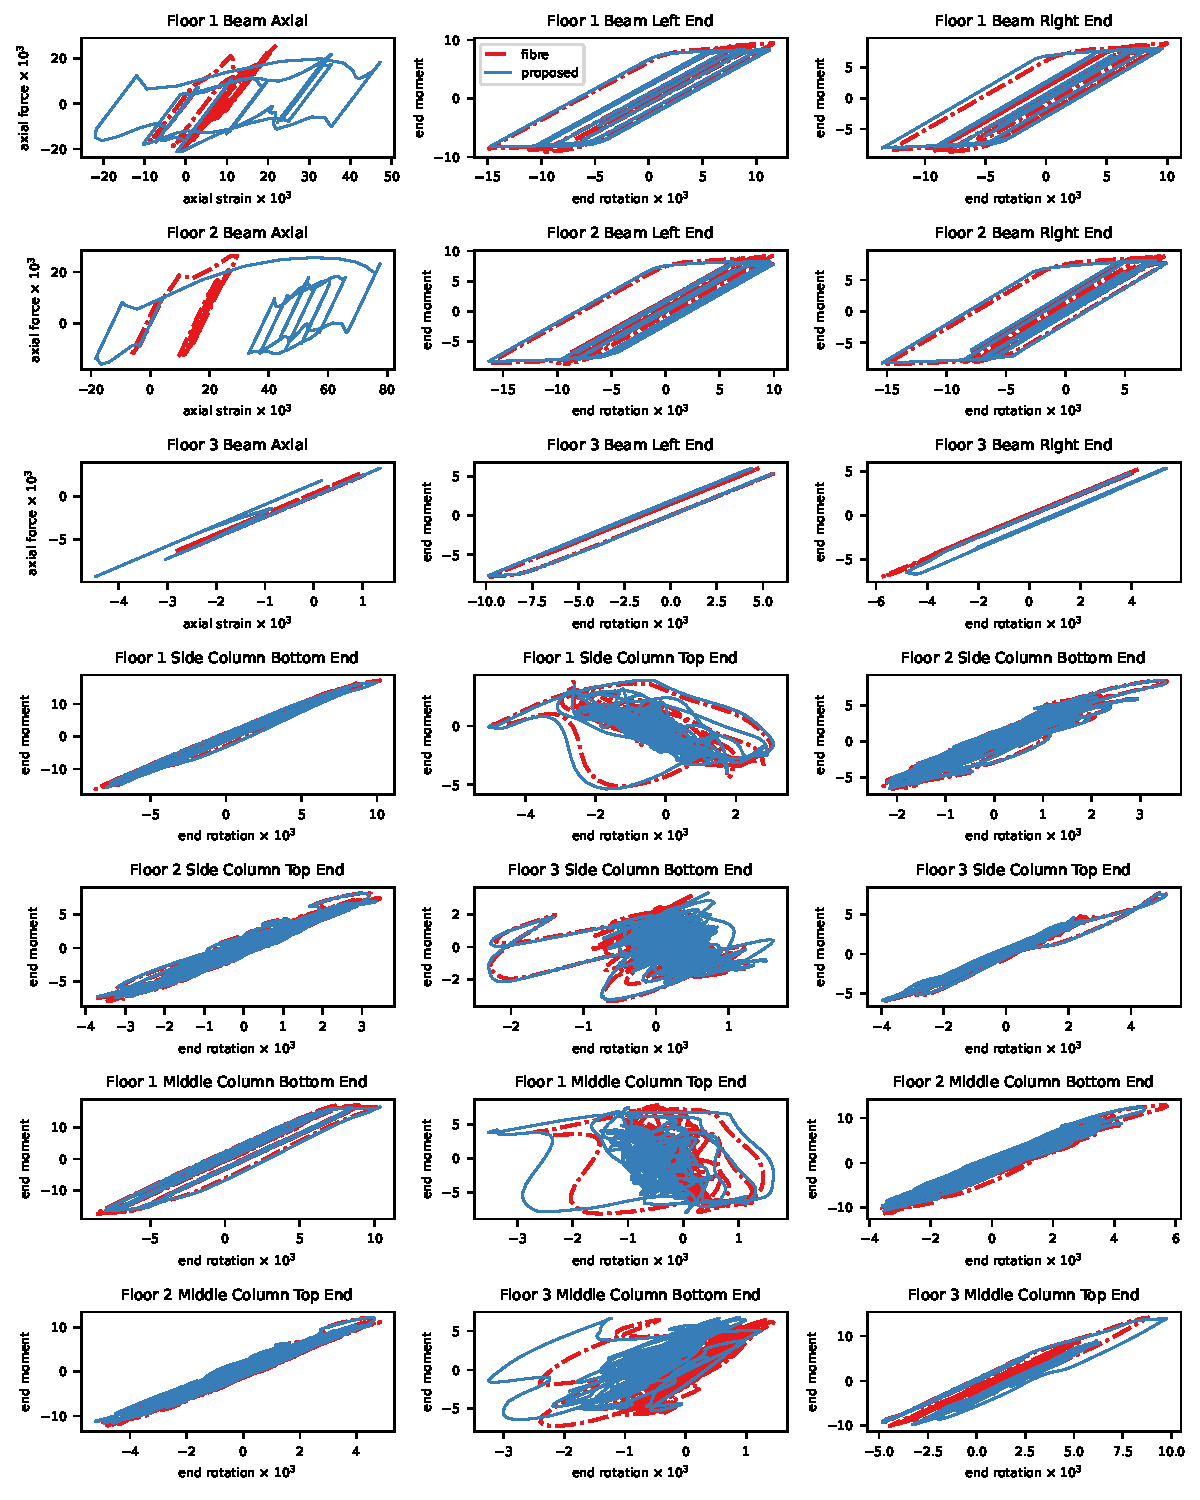
\includegraphics[width=.99\textwidth]{MODELS/FRAME/RESULT/FRAME.RESULT}
\caption{Hysteresis of frame members}\label{fig:hys}
\end{figure}
In terms of computational cost, for this specific structure, in a parallel context, performing a full response history analysis with the proposed element takes around \SI{30}{\percent} less wall clock time. Note that the number is indicative and may vary depending on different configurations. Excluding the time spent on solving the global matrix, the cost of which is not relevant to element formulations, the proposed element takes around \SI{80}{\percent} less time in terms of sole state determination. Given that the solution of the global matrix typically accounts for a significant portion of the overall computational time, a reduction of \SI{30}{\percent} is regarded as decent.

To close this example, the hysteresis of frame members is presented in \figref{fig:hys}.
It must be pointed out that frame end hysteresis ($\theta_z$-$M_z$) does not reflect whether the target end yields. See the discussion around \eqsref{eq:redefine}.
The responses of components that are not shown (such as the axial forces of middle columns) are purely elastic.

In general, both elements exhibit a comparable hysteresis pattern. As all beams yield, a beam--sway mechanism is formed. However, due to the sensitivity to plastic deformation, the centre of hysteresis may shift by varying amounts.

For a similar bending moment response, the proposed element tends to exhibit larger axial deformation of beams, suggesting that further calibration is necessary for the $N$-$M$ interaction surface. This disparity may arise from multiple sources, including insufficient integration points utilised in fibre elements, inaccurate section discretisation, and varying hardening behaviour attributed to different formulations.

If desired, analysts may perform calibration or implement more sophisticated hardening rules, such as the one presented in the appendix. Nonetheless, as these topics fall beyond the scope of this work, they are not discussed further.

It is worth mentioning that there is no intent to fine-tune the element behaviour to match experimental data on a designation-by-designation basis. Instead, the above structure is presented as a practical example to demonstrate that, without a complex calibration procedure, the proposed element can generate results with a certain level of confidence due to the correct formulation of hardening rules.

Upon comparison with the reference force-based element, it becomes apparent that the results obtained from both elements are similar. There is no plausible reason to indicate that one element is superior to the other. In specific circumstances where the overall response is governed by the strain--stress response at the material level, fibre models tend to necessitate fewer calibration efforts for different members. With the current model, it is required to calibrate $N$-$M$ interaction surfaces on a member-by-member basis.
\section{Conclusions}
In this work, the generalised plasticity theory is revisited and applied to conventional beam elements.
By using a revised yield function, which is able to capture the yielding of either end(s), we formulate an efficient concentrated plasticity beam element that supports the $N$-$M$ interaction, which allows the definition of flexible sectional responses.
The proposed formulation adopts sectional deformations and resultants as the basic quantities and determines the plastic state using a return mapping algorithm.
As evidenced by the frame example, the proposed formulation demonstrates a fairly moderate reduction in computational costs when compared to fibre elements for the presented relatively simple structure.
This renders it an effective and performant tool for simulating lumped plastic hinges at beam ends with zero hinge length.

By properly accounting for the special constraint that the axial force is unique but shared between two end nodes, the hardening behaviour is corrected.
The proposed element shows desired isotropic/kinematic hardening response.
The hardening parameters are now tightly associated with physical implications, making the calibration more reliable.
As the presented hardening laws are suitable for steel beams/columns, practical examples are presented to showcase that the proposed element can be used in response history analysis of steel frames without a complex calibration procedure of model parameters.
It is imperative to note that the exact plastic rules delineated in this study are exclusively applicable to a particular case of steel members with a bilinear material stress--strain law, and are not suitable for sections made of alternative materials, such as reinforced concrete.
Nevertheless, with the proposed formulation, other plastic rules and interaction surfaces can be adopted to simulate other types of frames.
The formulation itself does not impose any restrictions in this regard.
It provides an alternative to conventional beam elements with flexibility for response history analysis.

As sectional quantities are employed as the basic quantities, the corresponding calibration of model parameters (hardening rules and $N$-$M$ interactions) should be carried out based on the corresponding experimental data of member tests or accurate sectional analysis results (in absence of experimental data), if the proposed model is to be used in predictive simulations.

The proposed beam elements (both 2D and 3D versions) are implemented in \texttt{suanPan} \citep{Chang2022}, and all numerical examples are analysed using the same application.
\appendix
\section{Component Based Kinematic Hardening Rule}
Consider a 3D frame element with singly symmetric section geometry, as in general the shape factor, which corresponds to the saturation level defined in the kinematic hardening rule, would have different values along different axes, it is desired to assign different hardening rules for different components.

A simple modification of \eqsref{eq:nm_kin} can be expressed as
\begin{gather}
\dot{\overline{\bbeta}}=\begin{bmatrix}
K_{b,P}&\cdot&\cdot\\
\cdot&K_{b,M_z}&\cdot\\
\cdot&\cdot&K_{b,M_y}
\end{bmatrix}\dot{\overline{\be}^p}-\begin{bmatrix}
K_{a,P}&\cdot&\cdot\\
\cdot&K_{a,M_z}&\cdot\\
\cdot&\cdot&K_{a,M_y}
\end{bmatrix}\norm{\dot{\overline{\be}^p}}\overline{\bbeta}.
\end{gather}
The $K_a$ and $K_b$ pairs can be independently calibrated for each component to match the corresponding section properties of strong/weak axes.

Furthermore, consider an idealised bilinear material model, under pure axial deformation, the axial force resistance follows the material model and generates a bilinear response. However, under pure bending deformation, the end moment develops plasticity gradually and generates a non-linear response, which asymptotically approaches the plastic moment after yielding. One can set $K_{a,P}=0$, $K_{a,M_z}\neq0$ and $K_{a,M_y}\neq0$ so that axial back resistance evolves linearly while bending resistance evolves non-linearly. A graphical illustration of 2D elements is given in \figref{fig:nm_component_kin}.
\begin{figure}[htb]
\centering\footnotesize
\includegraphics[page=15]{PICCOLLECTION}
\caption{Different rules of kinematic hardening evolution of a 2D beam.}\label{fig:nm_component_kin}
\end{figure}
\section*{Data Availability Statement}
Some or all data, models, or code that support the findings of this study are available from the corresponding author upon reasonable request.
The corresponding model scripts are available online\footnote{\url{https://github.com/TLCFEM/nm-formulation}}.